\documentclass[conference,a4paper]{IEEEtran}

\usepackage[T1]{fontenc}
\usepackage{mathptmx}
\usepackage[top=2cm,bottom=2cm,left=2cm,right=1.5cm]{geometry}
\usepackage[pdftex]{graphicx}
\usepackage{amsfonts}
\usepackage{amssymb}
\usepackage{amsmath}
\usepackage{float}
\usepackage{graphicx,epsf}
\usepackage{booktabs}
\usepackage{datetime}
\graphicspath{{./pics/}}   

\begin{document}

\title{Report Subject \normalsize\vspace*{10pt} \\Kittikom Sangrit \\National Electronics and Computer Technology Center \\\vspace*{20pt} \today{}}

\maketitle

\begin{abstract}
Put your brief summary here. It should be less than 150 words.
Lorem ipsum dolor sit amet, consectetur adipiscing elit, sed do              
eiusmod tempor incididunt ut labore et dolore magna aliqua. Ut               
enim ad minim veniam, quis nostrud exercitation ullamco laboris..
\end{abstract}

\begin{IEEEkeywords}
keyword 1, keyword 2, keyword 3, keyword 4, keyword 5
\end{IEEEkeywords}

\section{Introduction}

The mass-energy equivalence can be stated mathematically as follows.
\begin{equation}
E = mc^2,
\label{eq1}
\end{equation}
where $E$ is the equivalent energy, $m$ is the mass, and $c$ is the speed of light.

\begin{equation}
A = \sum_{i=1}^{n}\left(\frac{\sqrt{\lambda_i}}{\epsilon+\Gamma^2_i\frac{\left(\Theta-\tau\right)}{\theta}}\right)^{0.8}.
\label{eq2}
\end{equation}

See Eq.\,(\ref{eq1}) and Eq.\,(\ref{eq2}), $\cdots$

A signal $F\!=\![f_0 \; f_1 \; f_2 \; ... \; f_{N-1}]^\textrm{T}$ of length $N\!>\!2$ is mapped to a matrix $\mathbf{X}$ of size $L\!\times\!K$, where $L$ is an positive integer less than $N$, and $K\!=\!N\!-\!L\!+\!1$. Note that the superscript $\text{T}$ denotes the transpose of a matrix.

\begin{equation}
\mathbf{X} = 
\left[ {\begin{array}{*{20}c}
   f_0 & f_1 & f_2 & \cdots & f_{K-1} \\
   f_1 & f_2 & f_3 & \cdots & f_{K} \\
   f_2 & f_3 & f_4 & \cdots & f_{K+1} \\
   \vdots & \vdots & \vdots & \ddots & \vdots \\
   f_{L-1} & f_L & f_{L+1} & \cdots & f_{N-1} \\
 \end{array} } \right].
\label{eq3}
\end{equation}

Each resultant matrix is mapped to a signal of length $N$ by diagonal averaging (Hankelization). The Hankelization of a matrix $\mathbf{Y}$ of size $L\!\times\!K$ to a signal $G\!=\![g_0 \; g_1 \; g_2 \; ... \; g_{N-1}]^\textrm{T}$ is defined by the following equation.
\begin{equation}
g_k =\left\{
\begin{array}{ll}
    \begin{array}{ll}
      \frac{1}{k+1}\displaystyle\sum_{m=1}^{k+1}y^*_{m,k-m+2}, & \quad\textrm{for} \quad 0 \leq k < L^*\!-\!1, \\
      \frac{1}{L^*}\displaystyle\sum_{m=1}^{L^*}y^*_{m,k-m+2}, & \quad\textrm{for} \quad L^*\!-\!1 \leq k < K^*, \\
      \frac{1}{N-k}\displaystyle\sum_{m=k-K^*+2}^{N-K^*+1}y^*_{m,k-m+2}, & \quad\textrm{for} \quad K^* \leq k < N,
    \end{array}
\end{array}
\right.
\label{eq4}
\end{equation}
where $y_{i\!j}$ is an element at the row $i$ and column $j$ of the matrix $\mathbf{Y}$, $L^* \!=\!\min(L,K)$, $K^*\!=\!\max(L,K)$, $y^*_{i\!j}\!=\!y_{i\!j}$ when $L\!<\!K$, and $y^*_{i\!j}\!=\!y_{\!j\!i}$ when $L\!\geq\!K$

\section{Section 2}
\subsection{Subsection Title}
\subsubsection{Subsubsection Title}
\subsubsection{Subsubsection Title}
\subsection{Subsection Title}

\section{Section 3}

An example of inserting a figure is shown in Fig.\,\ref{fig1}.

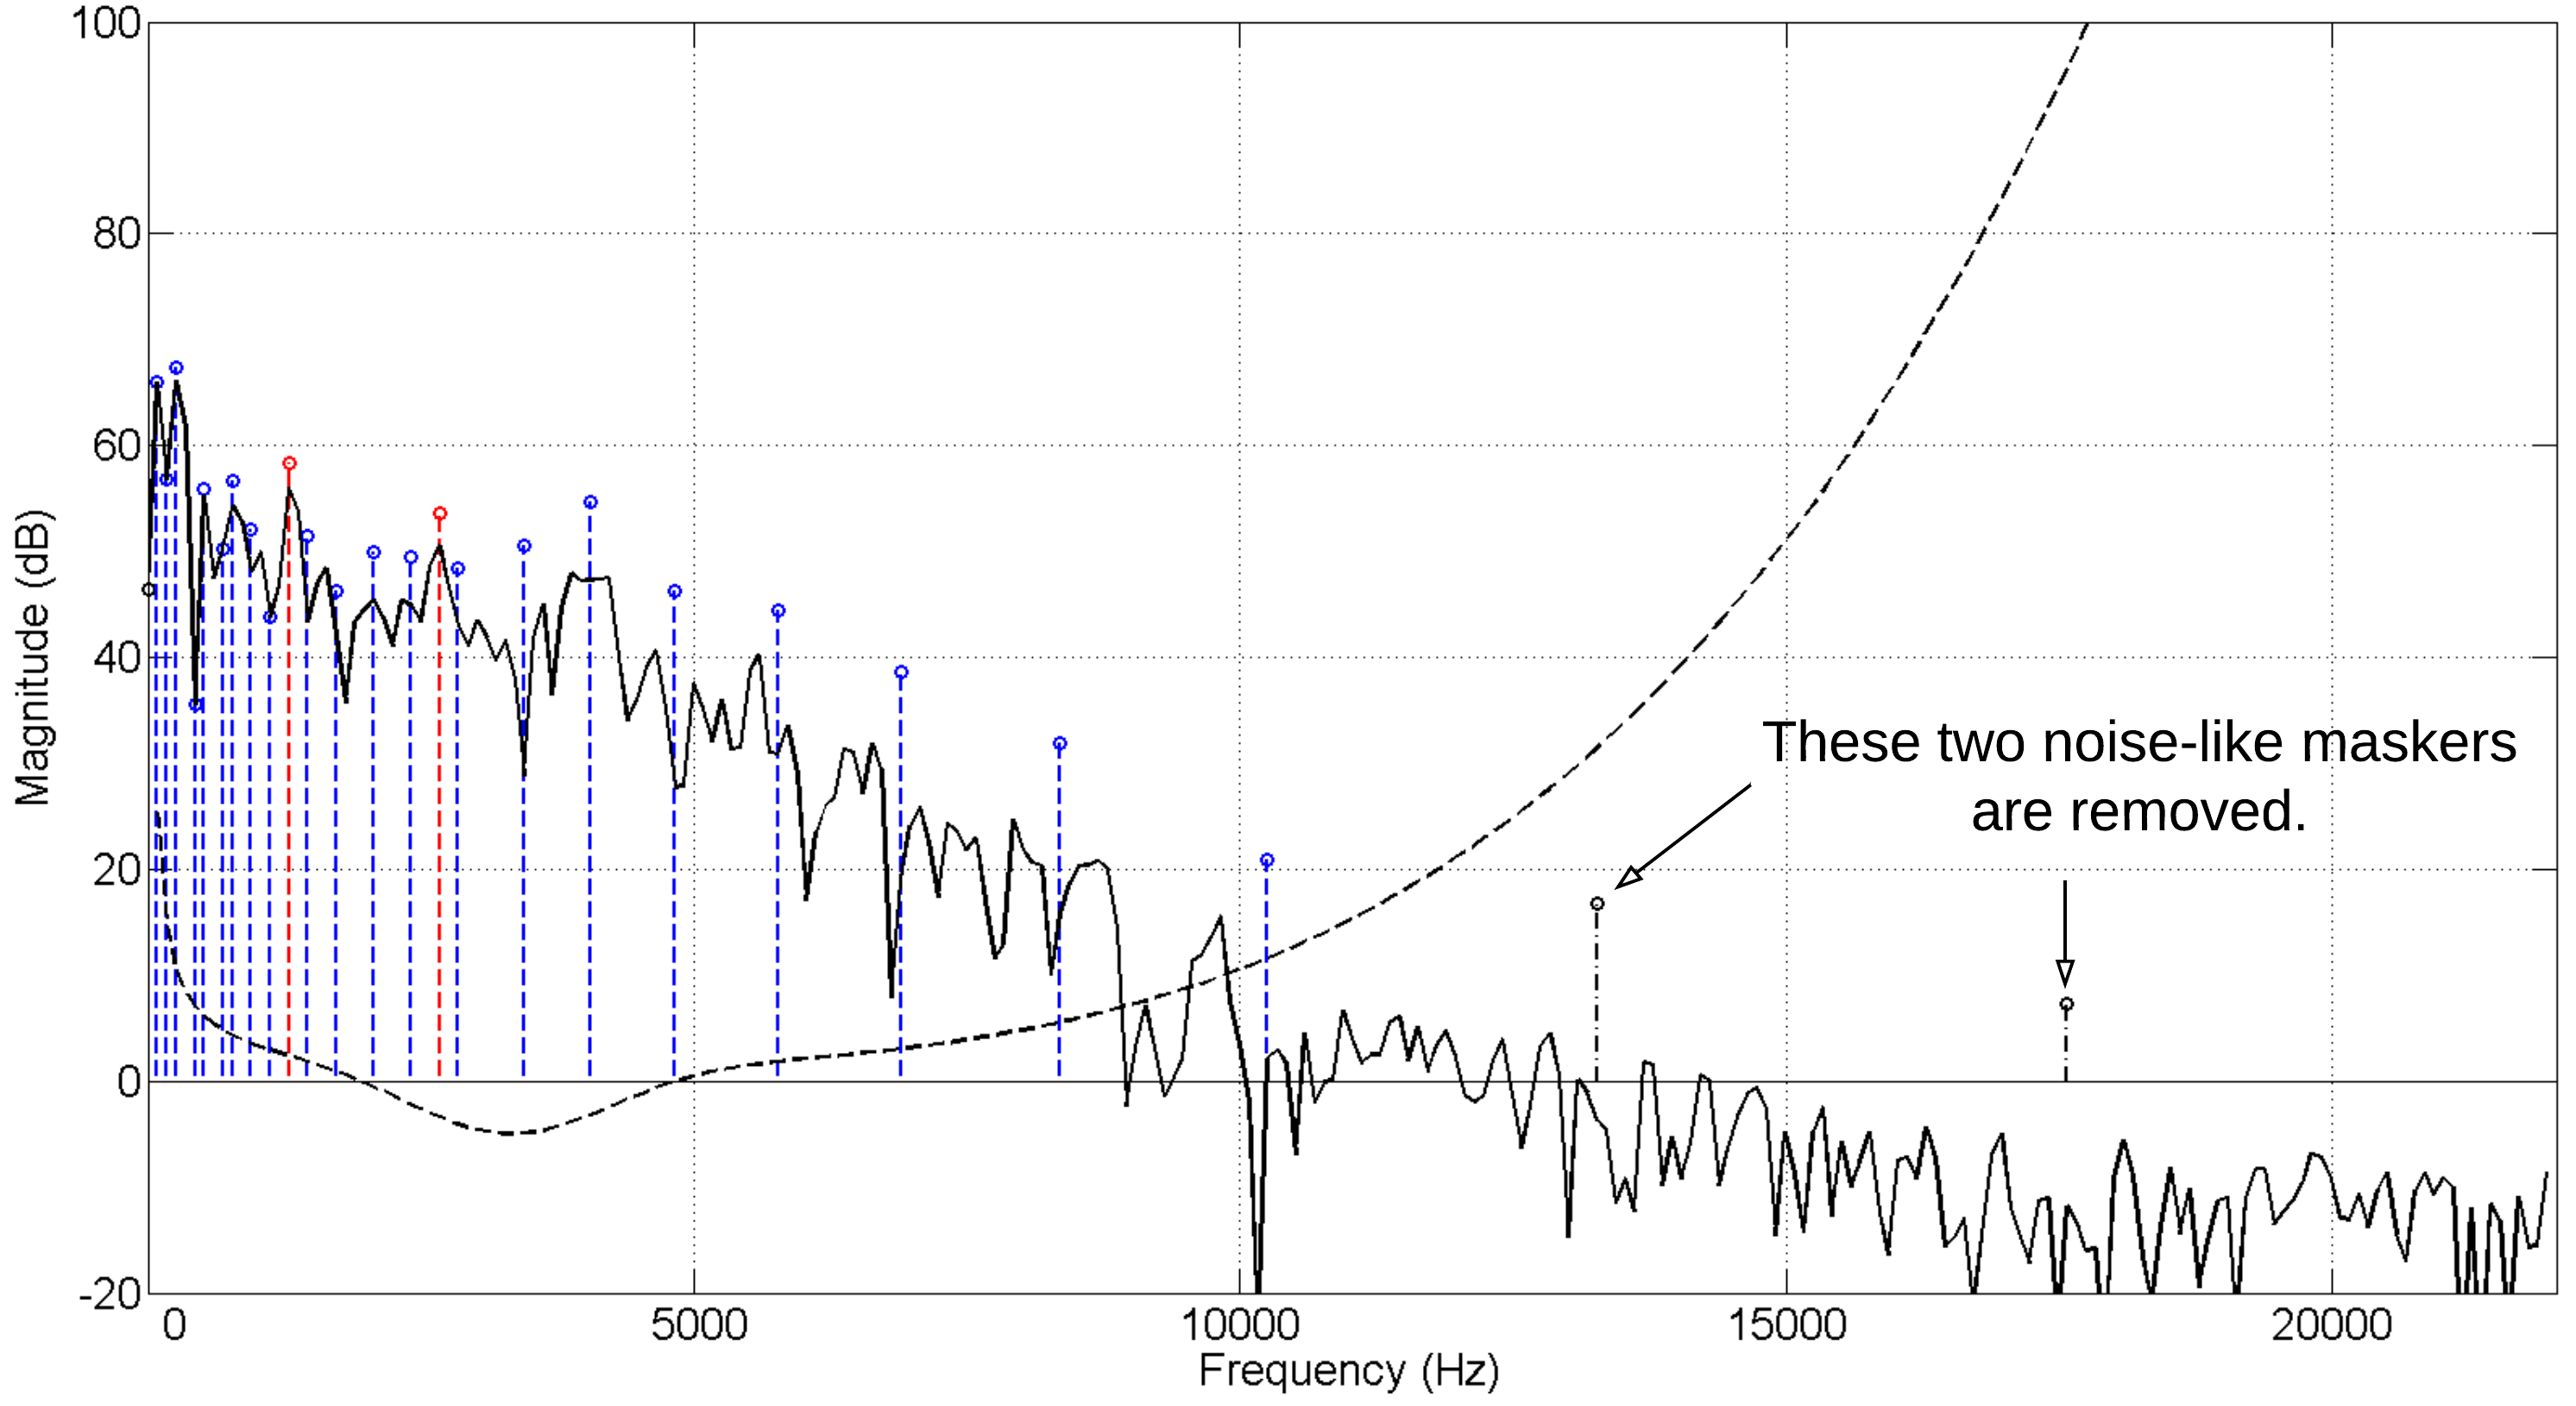
\includegraphics[width=1\linewidth]{graph.png}

To insert a table, see Table \ref{table1}. 

\begin{table}[h]
\centering
\caption{Table Caption}
\label{table1}
\begin{tabular}{@{}llcc@{}}
\toprule
\multicolumn{1}{c}{\textbf{}} & \hspace{1cm} & \textbf{X} & \textbf{Y} \\ \midrule
test table 1 &  & 123456.7 & 0.000001 \\
test table 2 &  & 7.654321 & 1.000002 \\ \bottomrule
\end{tabular}
\end{table}

Please visit: \texttt{http://www.tablesgenerator.com/}.

\section{Section 4}

It is easy to learn \LaTeX. It is easy to cite the bibliographies \cite{dutoit2009}\cite{craver2001}\cite{fallahpour2011}.

\section{Conclusion}
Lorem ipsum dolor sit amet, consectetur adipiscing elit, sed do              
eiusmod tempor incididunt ut labore et dolore magna aliqua. Ut               
enim ad minim veniam, quis nostrud exercitation ullamco laboris..

\begin{thebibliography}{1}

\bibitem{dutoit2009}
T.\,Dutoit and F.\,Marques, ``Applied Signal Processing: A MATLAB-Based Proof of Concept,'' {\em{Springer}}, 2009.  

\bibitem{craver2001}
S.\,A.\,Craver, M.\,Wu and B.\,Liu, ``What Can We Reasonably Expect from Watermarks?,'' Proc. {\em{IEEE Workshop on Application of Signal Processing to Audio and Acoustics,}}, 223--226, 2001. 

\bibitem{fallahpour2011}
M.\,Fallahpour and D.\,Megias, ``High Capacity Audio Watermarking Using the High Frequency Band of the Wavelet Domain,'' {\em{Multimedia Tools and Applications}}, Vol. \textbf{52}(2-3), 485--498, 2011.

\end{thebibliography}
\end{document}


